\documentclass[10pt,titlepage]{article}
\usepackage[english]{babel}
\usepackage[utf8]{inputenc}
\usepackage{algorithm}
\usepackage[noend]{algpseudocode}
\usepackage{amsmath,amsfonts,amsthm}
\usepackage{spverbatim}
\usepackage{listings}
\usepackage{xcolor}
\usepackage{pgfplots}
\usepackage[letterpaper, margin=1.25in]{geometry}
\usepackage{titlesec}
\usepackage{fancyhdr}
\usepackage{graphicx}
\usetikzlibrary{trees}
\usepackage[normalem]{ulem}
\useunder{\uline}{\ul}{}

\lstdefinestyle{mystyle}{
	keywordstyle=\color{blue},
	commentstyle=\color{red},
	stringstyle=\color{violet},
	basicstyle=\fontsize{12}{12},
	columns=fullflexible,
	breaklines=true
}

\titleformat{\section}
{\normalfont\Large\bfseries}{\thesection}{1em}{}[{\titlerule[0.8pt]}]
\lstset{style=mystyle}

\title{Low Level Design}

\author{Seth Williams, Abraham Sharum, Parker Fletcher, Bryson Dye \\\\ \\ Due Date: September 30, 2025 \\ Class: CS 40003 - Software Engineering}	

\lstset{style=mystyle}
\begin{document}
	\pagestyle{fancy}
	\fancyhead{}
	\fancyhead[LE,LO]{\textbf{CS 40003 - Software Engineering}}
	\fancyhead[RO,RE]{\textbf{Low Level Design}}
	\fancyfoot{}
	\fancyfoot[CE,CO]{\textbf{\thepage}}
	\maketitle
	
	\section*{Class Diagram}
	
	\begin{figure}[H]
		\centering
		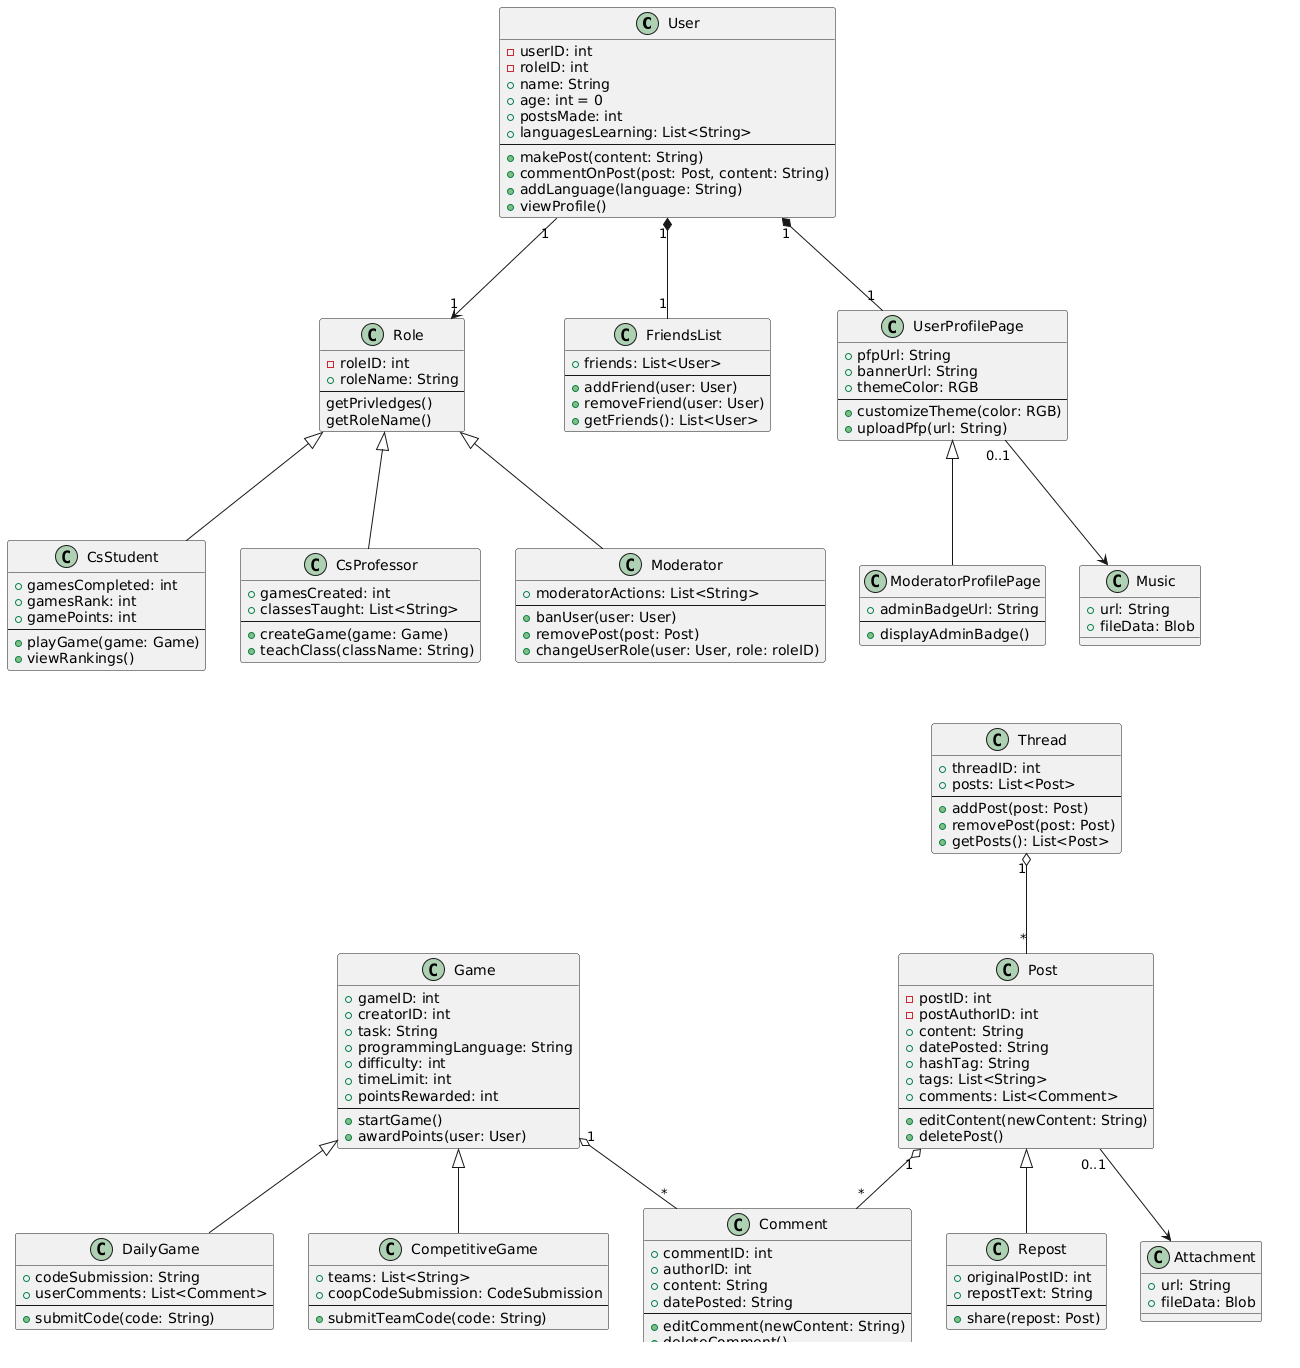
\includegraphics[width=\textwidth,height=0.6\textheight,keepaspectratio]{ClassDiagram.png}
		\caption{Class Diagram}
		\label{fig:class}
	\end{figure}
	
	\section*{Sequence Diagrams}
	
	\subsection*{User Sequence Diagram}
	
	\begin{figure}[H]
		\centering
		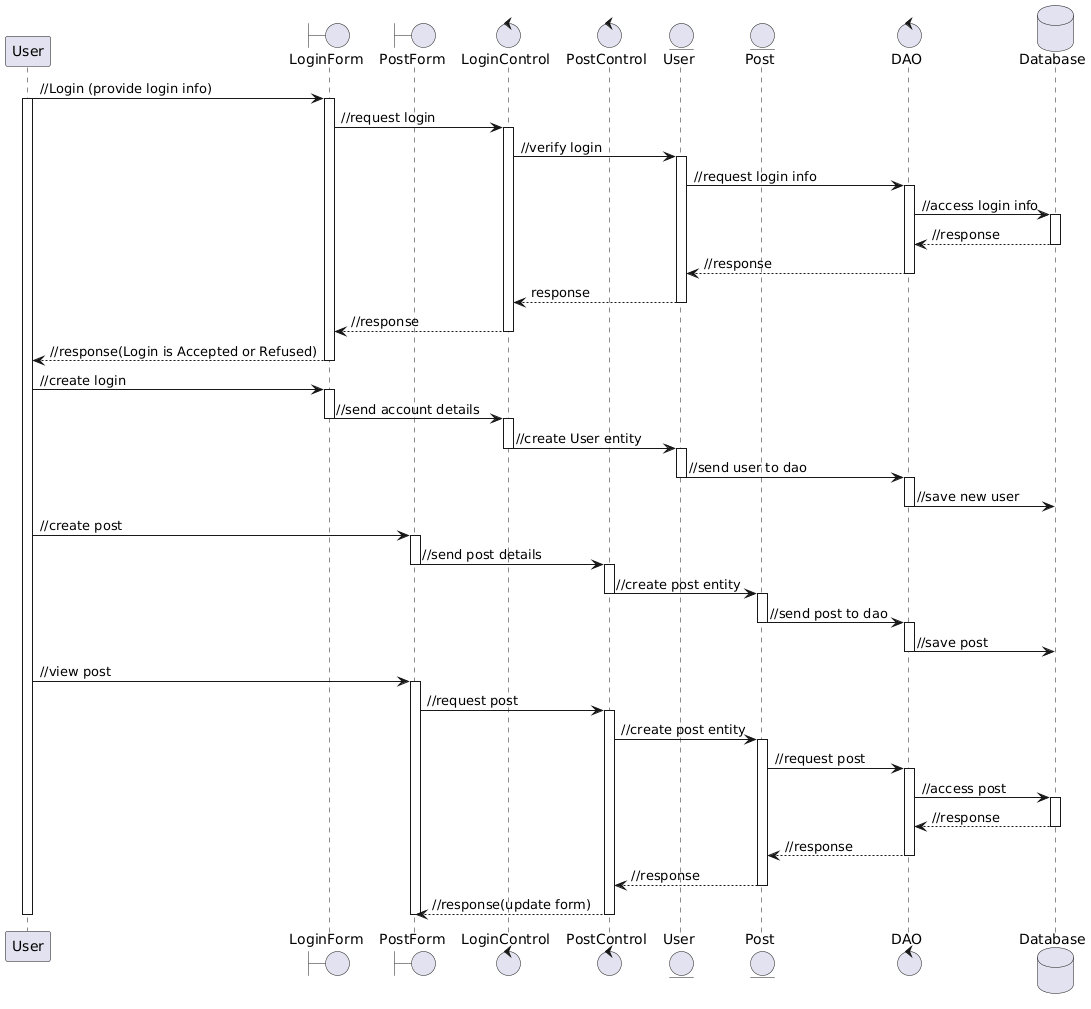
\includegraphics[width=\textwidth,height=0.6\textheight,keepaspectratio]{SequenceDiagram 1.png}
		\caption{User Sequence Diagram}
		\label{fig:User}
	\end{figure}
	
	\subsection*{Application Sequence Diagram}
	
	\begin{figure}[H]
		\centering
		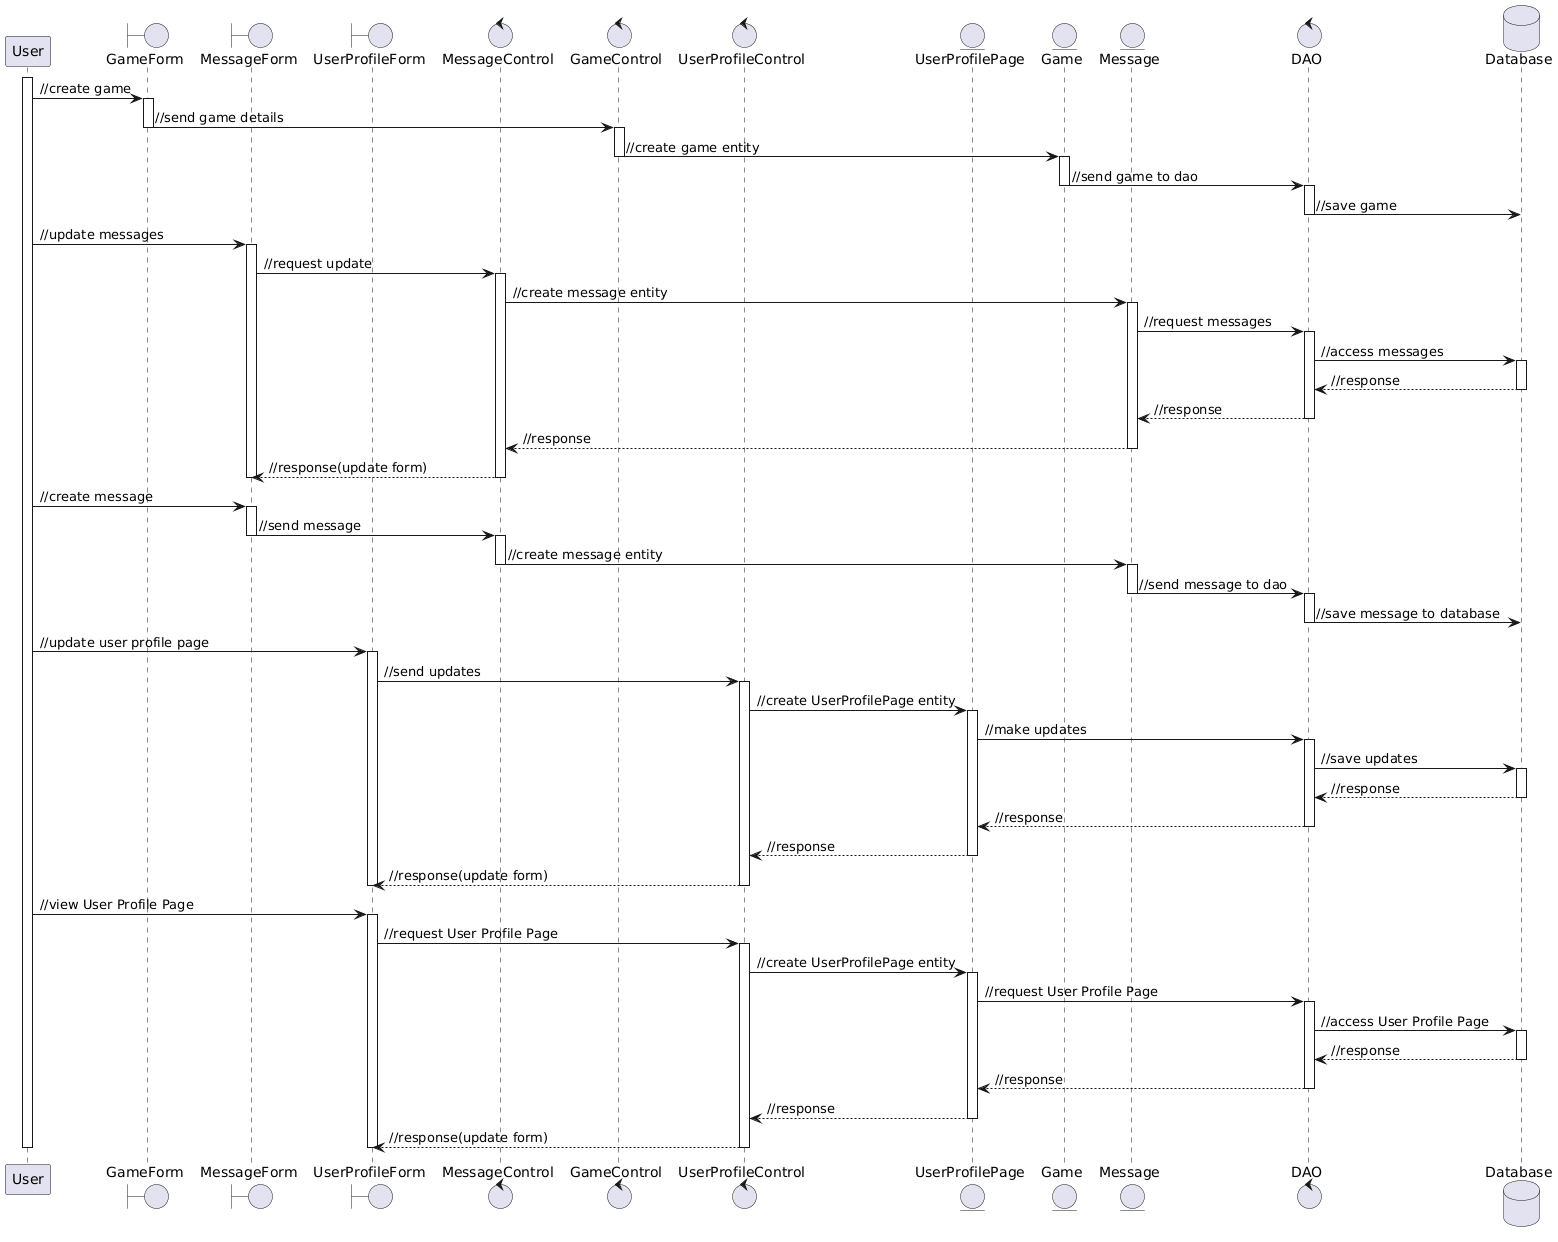
\includegraphics[width=\textwidth,height=0.6\textheight,keepaspectratio]{SequenceDiagram 2.png}
		\caption{Application Sequence Diagram}
		\label{fig:Application}
	\end{figure}
	
	\section*{Sate Diagram}
	
	\begin{figure}[H]
		\centering
		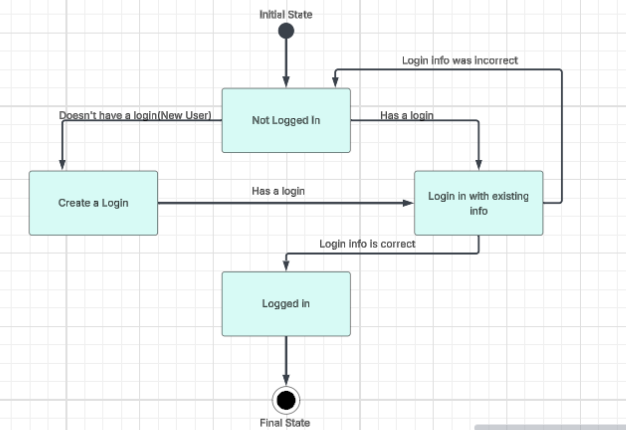
\includegraphics[width=\textwidth,height=0.6\textheight,keepaspectratio]{StateDiagram.png}
		\caption{State Diagram}
		\label{fig:State}
	\end{figure}
	
	\section*{Use Case Diagram}
	
	\begin{figure}[H]
		\centering
		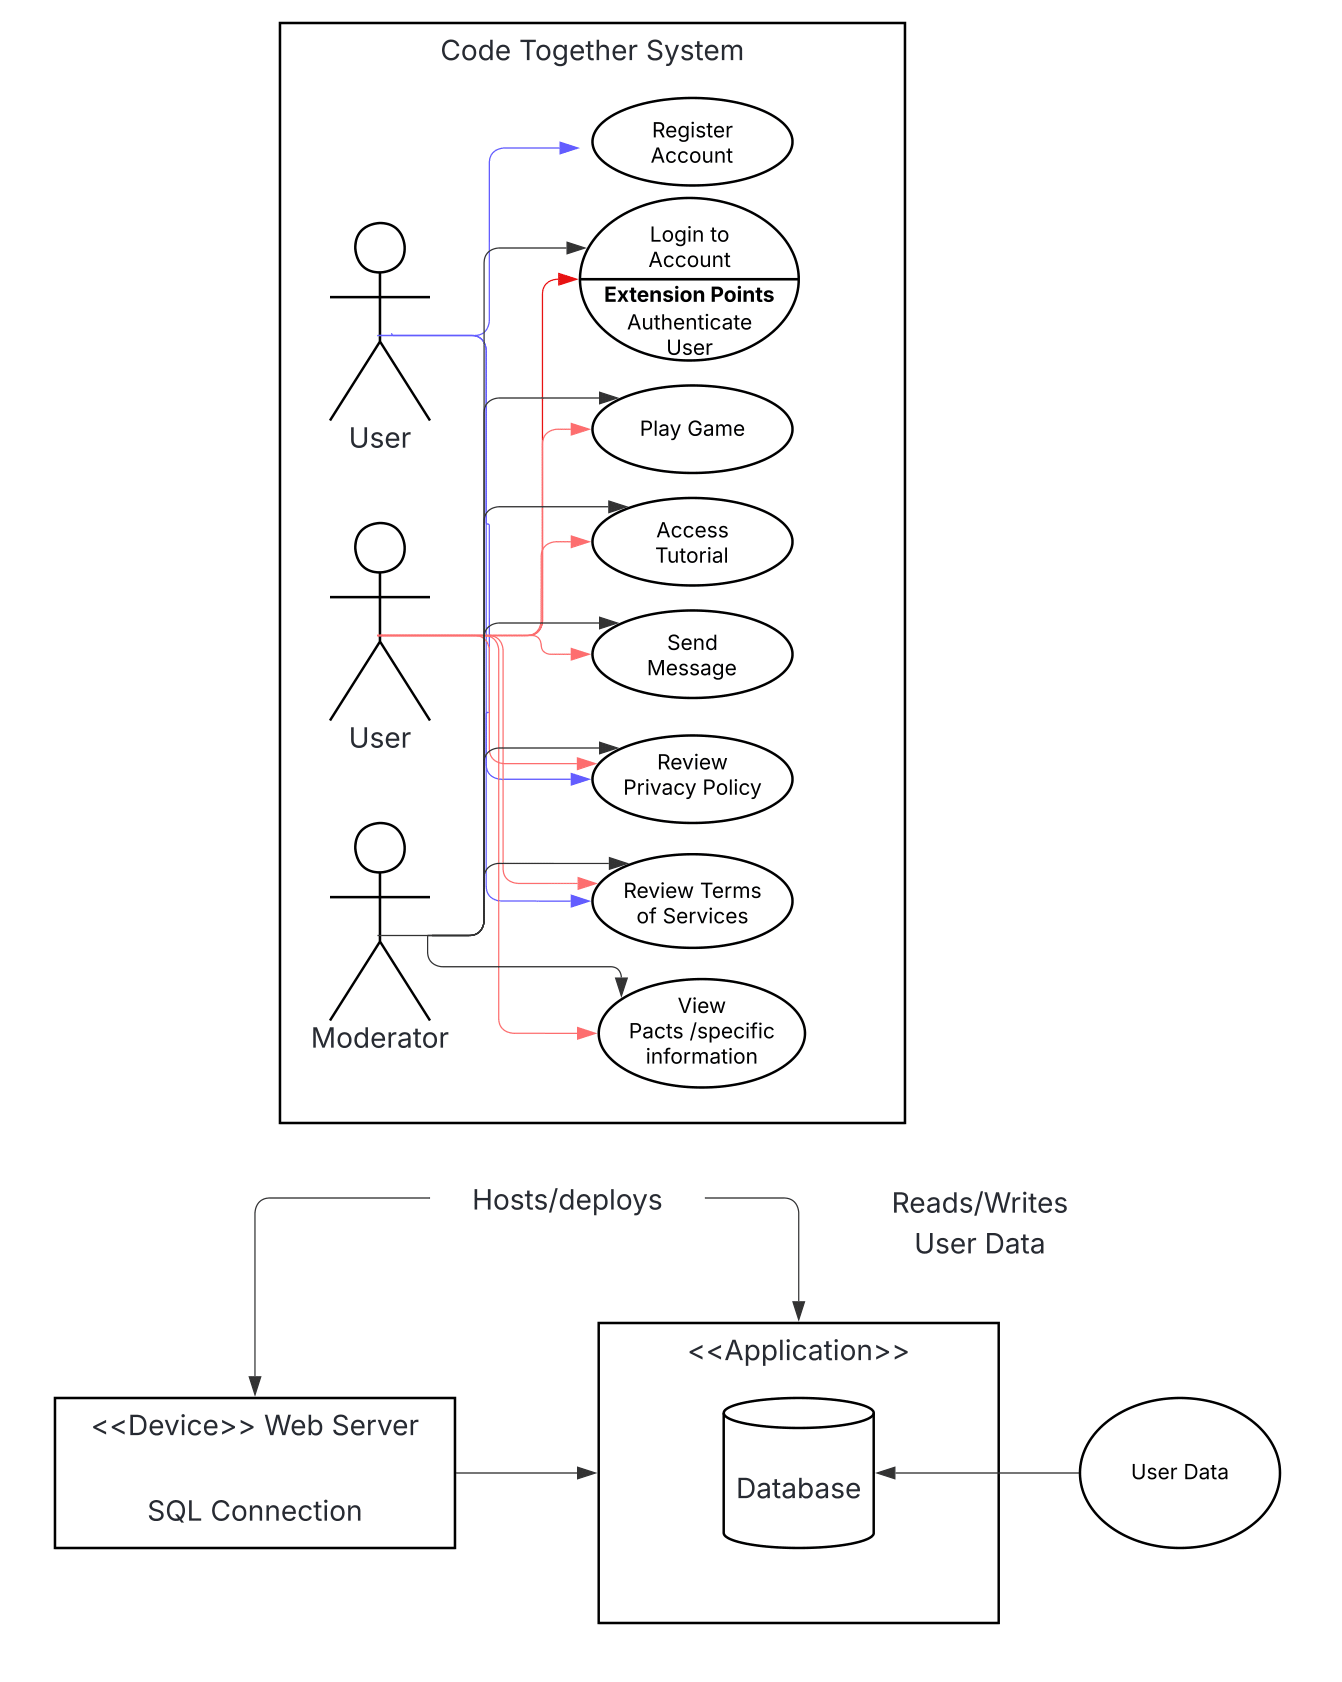
\includegraphics[width=\textwidth,height=0.6\textheight,keepaspectratio]{UseCaseDiagram.png}
		\caption{Use Case Diagram}
		\label{fig:Use Case}
	\end{figure}
	
	
	
	
\end{document}
